%%%%%%%%%%%%%%%%%%%%%%%%%%%%%%%%%%%%%%%%%%%%%%%%%%%%%%%%%%%%%%%
% Welcome to the MAT320 Homework template on Overleaf -- just edit your
% LaTeX on the left, and we'll compile it for you on the right.
%%%%%%%%%%%%%%%%%%%%%%%%%%%%%%%%%%%%%%%%%%%%%%%%%%%%%%%%%%%%%%%
% --------------------------------------------------------------
% Based on a homework template by Dana Ernst.
% --------------------------------------------------------------
% This is all preamble stuff that you don't have to worry about.
% Head down to where it says "Start here"
% --------------------------------------------------------------

\documentclass[12pt]{article}

\usepackage{graphicx}
\graphicspath{{./images/}}
\usepackage[margin=1in]{geometry} 
\usepackage{amsmath,amsthm,amssymb}
\usepackage{enumitem} % allows using letters in enumerate list environment

% source: https://stackoverflow.com/questions/3175105/inserting-code-in-this-latex-document-with-indentation

\usepackage{listings}
\usepackage{color}

\definecolor{dkgreen}{rgb}{0,0.6,0}
\definecolor{gray}{rgb}{0.5,0.5,0.5}
\definecolor{mauve}{rgb}{0.58,0,0.82}

\lstset{frame=tb,
	language=C, % language for code listing
	aboveskip=3mm,
	belowskip=3mm,
	showstringspaces=false,
	columns=flexible,
	basicstyle={\small\ttfamily},
	numbers=none,
	numberstyle=\tiny\color{gray},
	keywordstyle=\color{blue},
	commentstyle=\color{dkgreen},
	stringstyle=\color{mauve},
	breaklines=true,
	breakatwhitespace=true,
	tabsize=4
}

\newcommand{\N}{\mathbb{N}}
\newcommand{\Z}{\mathbb{Z}}

\newenvironment{ex}[2][Exercise]{\begin{trivlist}
		\item[\hskip \labelsep {\bfseries #1}\hskip \labelsep {\bfseries #2.}]}{\end{trivlist}}

\newenvironment{sol}[1][Solution]{\begin{trivlist}
		\item[\hskip \labelsep {\bfseries #1:}]}{\end{trivlist}}


\begin{document}

% --------------------------------------------------------------
%                         Start here
% --------------------------------------------------------------

\noindent Sergio Garcia Tapia \hfill

\noindent{\small Digital Design and Computer Architecture: RISC-V} \hfill 

\noindent\today

\begin{ex}{1.4} 
An analog voltage is in the range of 0-5 V. If it can be measured with an accuracy of $\pm$50 mV, at most how many bits of information does it convey?
\end{ex}

\begin{sol}\
	According to \emph{Section 1.3: Digital Abstraction}, the \emph{amount of information} $D$ in a discrete valued varaible with $N$ distinct states is measured in units of \emph{bits} as
	\[D=\log_2N \]
	There are 6 digits in the 1s place (0 through 5), 10 digits in the first decimal (0 through 10), and 6 digits in the second decimal place (0 through 5). Overall, that is $6\cdot 10\cdot 6$ states, or $N=360$. Therefore, at most $D=\log_2{360}=8.49$ bits of information are conveyed.
\end{sol}

\begin{ex}{1.5}
	A classroom has an old clock on the wall whose minute hand broke off.
	\begin{enumerate}[label=(\alph*)]
		\item If you can read the hour hand to the nearest 15 minutes, how many bits of information does the clock convey about the time?
		\item If you know whether it is before or after noon, how many additional bits of information do you know about the time?
	\end{enumerate}
\end{ex}
\begin{sol}\
	\begin{enumerate}[label=(\alph*)]
		\item Since an hour has 60 minutes, the described conditions means there are 4 distinguishable states per hour. Since a wall-clock is only able to distinguish between 12 hours in a day (not 24), there are $12\cdot 4=48$ total states. Therefore, the amount of information $D$ is $D=\log_2{48}=5.58$ bits of information.
		\item If we know that it is before noon or after noon, we have one additional bit of information. If we were to do the math, note that we would have double the states, so now we would have
		\[
		D=\log_2{48\cdot 2}=\log_2{48}+\log_2{2}=\log_2{48}+1
		\]
	\end{enumerate}
\end{sol}
\begin{ex}{1.6}
	The Babylonians developed the \emph{sexagesimal} (base 60) number system about 4000 years ago. How many bits of information is conveyed with one sexagesimal digit? How do you write the number the number $4000_{10}$ in sexagesimal?
\end{ex}

\begin{sol}\
	Since there are 60 values for a sexagesimal digit, a total of $D=\log_2{60}=5.91$ bits of information are conveyed. To write $4000_{10}$ in sexagesimal, we repeatedly divide by 60 and assign the remainder to the current bit, starting from the right.
	\begin{align}
		4000 &= 60\cdot 66+40\nonumber\\
		66&=60\cdot 1 + 6\nonumber
	\end{align}
	Hence,
	\begin{align}
		4000_{10}&=60\cdot (60\cdot 1+6)+40\nonumber\\
		&=60^2\cdot 1+60\cdot 6+60^{0}\cdot 40
	\end{align}
	Therefore, starting from the right, the first digit is 40, followed by 6, followed by 1.
\end{sol}

\begin{ex}{1.7}
	How many different numbers can be represented with 16 bits?
\end{ex}

\begin{sol}\
	Each bit has two possible values: 0 or 1. Therefore, with 6 bits, we have $2^{16}$ different numbers, which is 65,536 possible values.
\end{sol}

\begin{ex}{1.8}
	What is the largest unsigned 32-bit binary number?
\end{ex}

\begin{sol}
	If unsigned, the largest 32-bit binary number is represented by all 1s. This is precisely $2^{32}-1=4,294,967,295$, or about 4.3 billion.
\end{sol}

\begin{ex}{1.9}
	What is the largest 16-bit binary number that can be represented with:
	\begin{enumerate}[label=(\alph*)]
		\item unsigned numbers?
		\item two's complement numbers?
		\item sign/magnitude numbers?
	\end{enumerate}
\end{ex}

\begin{sol}\
	\begin{enumerate}[label=(\alph*)]
		\item $2^{16}-1=65,535$
		\item $2^{15}-1=32,767$
		\item $2^{15}-1=32,767$
	\end{enumerate}
\end{sol}

\begin{ex}{1.10}
	What is the largest 32-bit number that can be represented with
	\begin{enumerate}[label=(\alph*)]
		\item unsigned numbers?
		\item two's complement numbers?
		\item sign/magnitude numbers?
	\end{enumerate}
\end{ex}

\begin{sol}\
	\begin{enumerate}[label=(\alph*)]
		\item $2^{32}-1=4,294,967,295$, or about 4.3 billion
		\item $2^{31}-1=2,147,483,647$, or about 2.1 billion
		\item $2^{31}-1=2,147,483,647$, or about 2.1 billion
	\end{enumerate}
\end{sol}

\begin{ex}{1.11}
	What is the smallest (most negative) 16-bit number that can be represented with
	\begin{enumerate}[label=(\alph*)]
		\item unsigned numbers?
		\item two's complement numbers?
		\item sign/magnitude numbers?
	\end{enumerate}
\end{ex}

\begin{sol}\
	\begin{enumerate}[label=(\alph*)]
		\item 0 is the smallest; negative numbers are not represented in this system.
		\item $-2^{15}=-32,768$
		\item $-2^{15}+1=-32,767$
	\end{enumerate}
\end{sol}

\begin{ex}{1.12}
	What is the smallest (most negative) 32-bit number that can be represented with
	\begin{enumerate}[label=(\alph*)]
		\item unsigned numbers?
		\item two's complement numbers?
		\item sign/magnitude numbers?
	\end{enumerate}
\end{ex}

\begin{sol}\
	\begin{enumerate}[label=(\alph*)]
		\item 0 is the smallest; negative numbers are not represented in this system.
		\item $-2^{31}=-1=2,147,483,648$
		\item $-2^{31}+1=-1=2,147,483,647$
	\end{enumerate}
\end{sol}

\begin{ex}{1.13}
	Convert the following unsigned binary numbers to decimal. Show your work.
	\begin{enumerate}[label=(\alph*)]
		\item $1010_2$
		\item $110110_2$
		\item $11110000_2$
		\item $000100010100111_2$
	\end{enumerate}
\end{ex}

\begin{sol}\
	\begin{enumerate}[label=(\alph*)]
		\item $1010_2=2^{3}\cdot 1+2^{2}\cdot 0+2^{1}\cdot 1+2^{0}\cdot 0=8_{10}+2_{10}=10_{10}$
		\item $110110_2=2^{5}+2^{4}+2^{2}+2^{1}=32+16+4+2=54_{10}$
		\item $11110000_2=2^{7}+2^{6}+2^{5}+2^{4}=128+64+32+16=240_{10}$
		\item $000100010100111_2=2^{11}+2^7+2^5+2^2+2^1+2^0=2215_{10}$
	\end{enumerate}
\end{sol}

\begin{ex}{1.14}
	Convert the following unsigned binary numbers to decimal. Show your work.
	\begin{enumerate}[label=(\alph*)]
		\item $1110_2$
		\item $100100_2$
		\item $11010111_2$
		\item $011101010100100_2$
	\end{enumerate}
\end{ex}

\begin{sol}\
	\begin{enumerate}[label=(\alph*)]
		\item $1110_2=2^3+2^2+2^1=8+4+2=14_{10}$
		\item $100100_2=2^5+2^2=32+4=36_{10}$
		\item $11010111_2=2^7+2^6+2^4+2^2+2^1+2^0=215_{10}$
		\item $011101010100100_2=2^{13}+2^{12}+2^{11}+2^9+2^7+2^5+2^2=15,012_{10}$
	\end{enumerate}
\end{sol}

\begin{ex}{1.15} Repeat Exercise 1.13, but convert to hexadecimal.
\end{ex}

\begin{sol}\
	\begin{enumerate}[label=(\alph*)]
		\item $1010_2=\text{A}_{16}$
		\item $110110_2=(11_2)(0110_2)=36_{16}$
		\item $11110000_2=(1111)_2(0000)_2=\text{F}0_{16}$
		\item $000100010100111_2=(000)_2(1000)_2(1010)_2(0111)_2=(8\text{A}7)_{16}$
\end{enumerate}	
\end{sol}

\begin{ex}{1.16} Repeat Exercise 1.14, but convert to hexadecimal.
\end{ex}

\begin{sol}\
	\begin{enumerate}[label=(\alph*)]
		\item $1110_2=\text{E}_{16}$
		\item $100100_2=(10)_2(0100)_2=24_{16}$
		\item $11010111_2=(1101)_2(0111)_2=\text{D}7_{16}$
		\item $011101010100100_2=(011)_2(1010)_2(1010)_2(0100)_2=\text{3AA4}_{16}$
	\end{enumerate}	
\end{sol}

\begin{ex}{1.17} Convert the following hexadecimal numbers to decimal. Show your work.
	\begin{enumerate}[label=(\alph*)]
		\item $\text{A5}_{16}$
		\item $\text{3B}_{16}$
		\item $\text{FFFF}_{16}$
		\item $\text{D000000}_{16}$
	\end{enumerate}
\end{ex}

\begin{sol}\
	\begin{enumerate}[label=(\alph*)]
		\item $\text{A5}_{16}=16^1\cdot 10+16^0\cdot 5=160+5=165_{10}$
		\item $\text{3B}_{16}=16^{1}\cdot 3+16^{0}\cdot 11=48+11=59_{10}$
		\item $\text{FFFF}_{16}=16^{3}\cdot 15+16^{2}\cdot 15+16^{1}\cdot 15+16^{0}\cdot 15=235,929,855_{10}$
		\item $\text{D0000000}_{16}=16^{7}\cdot 13=3,489,660,928_{10}$
	\end{enumerate}	
\end{sol}

\begin{ex}{1.18} Convert the following hexadecimal numbers to decimal. Show your work.
	\begin{enumerate}[label=(\alph*)]
		\item $\text{4E}_{16}$
		\item $\text{7C}_{16}$
		\item $\text{ED3A}_{16}$
		\item $\text{403FB001}_{16}$
	\end{enumerate}
\end{ex}

\begin{sol}\
	\begin{enumerate}[label=(\alph*)]
		\item $\text{4E}_{16}=16^{1}\cdot 4+16^{0}\cdot 14=78_{10}$
		\item $\text{7C}_{16}=16^1\cdot 7+16^{0}\cdot 12=124_{10}$
		\item $\text{ED3A}_{16}=16^{3}\cdot 14+16^{2}\cdot 13+16^{1}\cdot 3+16^{0}\cdot 10=60,730_{10}$
		\item $\text{403FB001}_{16}=16^7\cdot 4+16^5\cdot 3+16^4\cdot 15+16^3\cdot 11+16^0\cdot 1=1,077,915,664_{16}$
	\end{enumerate}
\end{sol}

\begin{ex}{1.19} Repeat exercise 1.17, but convert to unsigned binary.
\end{ex}

\begin{sol}\
	\begin{enumerate}[label=(\alph*)]
		\item $\text{A5}_{16}$: Since $A_{16}=1010_{2}$ and $5_{16}=0101_{2}$, we concatenate them to get $10100101_2$.
		\item $\text{3B}_{16}$: Concatenate $0011_2$ and $1011_2$ to get $00111011_2=111011_2$.
		\item $\text{FFFF}_{16}=1111111111111111_2$
		\item $\text{D000000}_{16}=1101000000000000000000000000_2$
\end{enumerate}
\end{sol}

\begin{ex}{1.20} Repeat exercise 1.18, but convert to unsigned binary.
\end{ex}

\begin{sol}\
	\begin{enumerate}[label=(\alph*)]
		\item $\text{4E}_{16}=$ $0100 1110_2$
		\item $\text{7C}_{16}=0111 1100_2$
		\item $\text{ED3A}_{16}$: Concatenate $\text{E}_{16}=1110_2$, $\text{D}_{16}=1101_2$, $\text{3}_{16}=0011_2$ and $\text{A}_{16}=1010_2$.
		\item $\text{403FB001}_{16}$: Concatenate $4_{16}=0100_2$, $0_{16}=0000_2$, $3_{16}=0011_2$, $\text{F}_{16}=1111_2$, $\text{B}_{16}=1011_{2}$, $0_{16}=0000$, $0_{16}=0000$, and $1_{16}=0001_2$:
		\[
		0100000000111111101000000000001_2
		\]
	\end{enumerate}
\end{sol}

\begin{ex}{1.21}
	Convert the following two's complement binary numbers to decimal.
	\begin{enumerate}[label=(\alph*)]
		\item $1010_2$
		\item $110110_2$
		\item $01110000_2$
		\item $10011111_2$
	\end{enumerate}
\end{ex}

\begin{sol}\
	\begin{enumerate}[label=(\alph*)]
		\item $1010_2$: Since this is a two's complement binary representation, the most significant bit represents the sign. Since the most significant bit is a 1, this is a negative number. To find the magnitude, we compute its two's complement by inverting its bits and adding 1:
		\[
		1010 \to 0101_2 + 1_2\to 0110_2=6_{10}
		\]
		Hence, the decimal equivalent is $-6_{10}$.
		\item $110110_2$: This is also negative. Its two's complement is:
		\[
		110110_2\to 001001_2+1_2\to 001010_2=2^{3}+2^{1}=10_{10}
		\]
		The decimal equivalent is thus $-10_{10}$.
		\item $01110000_2$: This time, the most significant bit is 0, so this number is positive. We do not have to find the two's complement this time, and obtain:
		\[
		2^{6}+2^{5}+2^{4}=112
		\]
		The decimal equivalent is $112_{10}$.
		\item $10011111_2$: This number is negative because of its most significant bit being 1. We find the two's complement:
		\[
		10011111_2\to01100000_2+1_2\to01100001_2=2^{6}+2^{5}+2^{0}=97_{10}
		\]
		The decimal equivalent is $-97_{10}$.
	\end{enumerate}
\end{sol}

\begin{ex}{1.22}
	Convert the following two's complement binary numbers to decimal.
	\begin{enumerate}[label=(\alph*)]
		\item $1110_2$
		\item $100011_2$
		\item $01001110_2$
		\item $10110101_2$
	\end{enumerate}
\end{ex}

\begin{sol}\
	\begin{enumerate}[label=(\alph*)]
		\item $1110_2$: Since the msb is 1, this number is negative. Its two's complement is:
		\[
		1110_2\to 0001_2+1_2\to0010_2=2_{10}
		\]
		The decimal equivalent is $-10_{2}$.
		\item $100011_2$: The msb is 1, so this number is negative. Its two's complement is:
		\[
		100011_2\to 011100_2+1_2\to 011101_2=2^{4}+2^{3}+2^{2}+2^{0}=29_{10}
		\]
		The decimal equivalent is $-29_{10}$.
		\item $01001110_2$: Since the msb is 0, this number is positive. Calculating the two's complement is not necessary, and we can start with the conversion:
		\[
		2^{6}+2^{3}+2^{2}+2^{1}=78_{10}
		\]
		\item $10110101_2$: The msb is 1, so this number is negative. Its two's complement is
		\[
		10110101_2\to 01001010_2+1_2\to01001011_2=2^{6}+2^{3}+2^{1}+2^{0}=75_{10}
		\]
		Its decimal equivalent is $-75_{10}$.
	\end{enumerate}
\end{sol}

\begin{ex}{1.41}
	How many 5-bit two's complement numbers are greater than 0? How many are less than 0? How would your answers differ for sign/magnitude numbers?
\end{ex}

\begin{sol}
	There are $2^{5}=32$ numbers in a 5-bit two's complement system. Of these, half (16) are negative. Therefore, there are 15 numbers greater than 0. If it were sign/magnitude, we would have 15 numbers greater than 0, and 15 less than 0, with the remaining two being -0 and +0.
\end{sol}

\begin{ex}{1.42}
	How many 7-bit two's complement numbers are greater than 0? How many are less than 0? How would your answers differ for sign/magnitude numbers?
\end{ex}

\begin{sol}
	There are $2^{7}=128$ numbers in a 5-bit two's complement system. Of these, half (64) are negative. Therefore, there are 63 numbers greater than 0. If it were sign/magnitude, we would have 63 numbers greater than 0, and 63 less than 0, with the remaining two being -0 and +0.
\end{sol}

\begin{ex}{1.43}
	How many bytes are in a 32-bit word? How many nibbles are in the 32-bit word?
\end{ex}

\begin{sol}
	A byte is 8 bits. Therefore, a 32-bit word has 4 bytes. A nibble is 4 bits, which represents one hexadecimal. THEREFORE, A 32-bit word has 8 nibbles.
\end{sol}

\begin{ex}{1.44}
	How many bytes are in a 64-bit word?
\end{ex}

\begin{sol}
	There 8 bytes in a 64-bit word.
\end{sol}

\begin{ex}{1.45}
	A particular DSL modem operates at 768 kbits/sec. How many bytes can it receive in 1 minute?
\end{ex}

\begin{sol}
	Since 768 bits is equivalent to 96 bytes, this is equivalent to 96 kilo bytes per second. Multiplying by 60, we get 5,760 kilo bytes per minute, or 5.76 mega bytes per minute, or 5,760,000 bytes in 1 minute.
\end{sol}

\begin{ex}{1.46}
	USB 3.0 can send data at 5 Gbits/sec. How many bytes can it send in 1 minute?
\end{ex}

\begin{sol}
	We multiply by 60 obtain 300 Gbits in one minute, or 300,000,000,000 bits, which is equivalent to 37,500,000,000 bytes.
\end{sol}

\begin{ex}{1.47}
	Hard drive manufacturers use the term ``megabyte'' to mean $10^6$ bytes and ``gigabyte" to mean $10^9$ bytes. How many real GBs (i.e., GiBs) of music can you store on a 50 GB hard drive?
\end{ex}

\begin{sol}
	Since a manufacturer means 50 gigabyte, this means $50\cdot 10^9$ bytes. However, since 1 GiB=1024MiB, and 1 MiB=1024 KiB, and 1 KiB=1024 bytes, we divide this by $(1024)^3$ to obtain approximately $46.6$ GiB.
\end{sol}

\begin{ex}{1.48}
	Estimate $2^{31}$ without using a calculator.
\end{ex}

\begin{sol}
	Since $2^{10}\approx 1,000$, $2^{20}\approx 1,000,000$, and $2^{30}\approx 1,000,000,000$, it follows that $2^{31}\approx 2,000,000,000$, or $2$ billion.
\end{sol}

\begin{ex}{1.49}
	A memory on the Pentium II microprocessor is organized as a rectangular array of bits with $2^8$ rows and $2^9$ columns. Estimate how many bits it has without using a calculator.
\end{ex}

\begin{sol}
	The memory has $2^{8}\cdot 2^{9}=2^{17}$ bits. Since $2^{10}\approx 1,000$ and $2^{7}=128$, this amounts to about $128,000$ bits, or $128$ kbits.
\end{sol}

\begin{ex}{1.52}
	Perform the following additions of unsigned binary numbers. Indicate whether the sum overflows a 4-bit result.
	\begin{enumerate}[label=(\alph*)]
		\item $1000_2+0100_2$
		\item $1101_2+1011_2$
	\end{enumerate}
\end{ex}

\begin{sol}\
	\begin{enumerate}[label=(\alph*)]
		\item
		\begin{center}
			\begin{tabular}{c@{\,}c@{\,}c@{\,}c@{\,}c@{\,}}
				& 1 & 0 & 0 & 0 \\
				+ & 0 & 1 & 0 & 0 \\
				\hline
				& 1 & 1 & 0 & 0
			\end{tabular}
		\end{center}
		The result does not overflow.
		\item
		\begin{center}
			\begin{tabular}{c*{5}{@{\,}c}}
				& 1 & 1 & 0 & 1 \\
				+ & 1 & 0 & 1 & 1 \\
				\hline
				1& 1& 0& 0& 0
			\end{tabular}
		\end{center}
		The result overflows.
	\end{enumerate}
\end{sol}

\begin{ex}{1.53}\
	\begin{enumerate}[label=(\alph*)]
		\item $10011001_2+01000100_2$
		\item $11010010_2+10110110_2$
	\end{enumerate}
\end{ex}

\begin{sol}\
	\begin{enumerate}[label=(\alph*)]
		\item The result does not overflow:
		\begin{center}
			\begin{tabular}{c*{8}{@{\,}c}}
				& 1 & 0 & 0 & 1 & 1 & 0 & 0 & 1 \\
		    +   & 0 & 1 & 0 & 0 & 0 & 1 & 0 & 0 \\
				\hline
				& 1 & 1 & 0 & 1 & 1 & 1 & 0 & 1
			\end{tabular}
		\end{center}
		\item The result overflows:
		\begin{center}
			\begin{tabular}{c*{8}{@{\,}c}}
					& 1 & 1 & 0 & 1 & 0 & 0 & 1 & 0 \\
				+   & 1 & 0 & 1 & 1 & 0 & 1 & 1 & 0 \\
				\hline
					& 0 & 1 & 1 & 0 & 1 & 0 & 0 & 0
			\end{tabular}
		\end{center}
	\end{enumerate}
\end{sol}

\begin{ex}{1.66}
	A flying saucer crashes in a Nebraska cornfield. The FBI investigates the wreckage and finds an engineering manual containing an equation in the Martian number system: 325+42=411. If this equation is correct, how many fingers would you expect martians to have?
\end{ex}

\begin{sol}
	The equation is true in base 6. Therefore, martians likely have 6 fingers.
\end{sol}

\begin{ex}{1.67}
	Ben Bitdiddle and Alyssa P. Hacker are having an argument. Ben says, `All integers greater than zero and exactly divisible by six have exactly two 1's in their binary representation." Alyssa disagrees. She says, ``No, but all such numbers have an even number of 1's in their binary representation". Do you agree with Ben or Alyssa or both or neither? Explain
\end{ex}

\begin{sol}
	We can experiment by writing some multiples of $6_{10}$ in binary. Certainly:
	\[
	6_{10}=110_2,\quad 12_{10}=1100, \quad 18_{10}=10010_2,\quad 24_{10}=11000_2,\quad 30_{10}=11110_{2}
	\]
	Since $30_{10}$ has more than two 1's, it turns out that Ben is wrong. We continue:
	\[
	36_{10}=100100_2,\quad 42_{10}=101010_2
	\]
	Given $42_{10}$ has three 1 bits, it turns out Alyssa is wrong, too.
\end{sol}

\begin{ex}{1.68}
	Ben Bitdiddle and Alyssa P. acker are having another argument. Ben says, ``I can get the two's complement of a number by subtracting 1, then inverting all the bits of the result." Alyssa says, ``No, I can do it by examining each bit of the number, starting with the least significant bit. When the first 1 is found, invert each subsequent bit." Do you agree with Ben or Alyssa or both or neither? Explain.
\end{ex}

\begin{sol}
	The two's complement of an N-bit number is obtained by subtracting the number from $2^N$. This number by an $(N+1)$-bit number with a $1$ in the most significant bit and 0 everywhere else. It can be obtained by adding $1$ to an $N$-bit $-1$ (represented by all 1 bits). Hence, the $N$-bit two's complement of $x$ is
	\[
	2^{N}-x=(11\cdots1 + 1) - x=(11\cdots 1 - x)  + 1
	\]
	In words, we invert the bits of $x$ (by subtracting it from $-1$) and then add $1$. Ben's description, subtracting $1$ and then inverting the bits of the result, is essentially:
	\[
	1-(x-1)=x + 2
	\]
	This leads to an incorrect answer. To demonstrate, given the 4-bit $1001_2$, two's complement is
	\[
	1001_2\to 0110_2 + 1\to 0111_2
	\]
	According to Ben's method, first we subtract 1 (with overflow):
	\[
	1001_2\to (1001_2-1)=1001_2+1111_2\to 1100_2
	\]
	and then inverting its bits we get $0011_2$, which is not correct. Alyssa's method, however, works correctly on this number, and it holds true. Suppose we have a nonzero, $N$-bit binary number, which therefore has a least significant 1-bit. Since finding the two's complement involves inverting all the bits and then adding 1, this means the rightmost 0 inverts to 1, and adding 1 to it inverts it back to 0, with a 1 carried to the next place. This happens for all 0's to the right of the least significant 1-bit. The least significant 1 is inverted to a 0, and when the carry bit reaches it, it becomes 1, but this time there is no carry. Therefore, all the bits to the left of it are unaffected after the bit inversion operation.
\end{sol}

\begin{ex}{1.69}
	Write a program in your favorite language (e.g., C, Java, Perl) to convert numbers from binary to decimal. The user should type in an unsigned binary number. The program should print the decimal equivalent.
\end{ex}

\begin{sol}\
	
	The following standalone C program, \texttt{binarytodecimal.c}, does the job. Instead of accepting command-line arguments, it prompts the user for a binary string, and upon receiving a valid input, it outputs the decimal result.
	\begin{lstlisting}
#include <stdio.h> /* printf, getchar, EOF */
#include <ctype.h> /* isspace */
#define MAXBITS 64

int readbits(char s[]);
unsigned long bintodecimal(char *s);

/* read unsigned binary number with up MAXBITS bits and display its decimal value */
int main(int argc, char *argv[])
{
	char s[MAXBITS + 1];
	
	printf("Enter an %d-bit binary number: ", MAXBITS);
	if (!readbits(s))
	return 1;	/* exit unsuccessfully */
	
	unsigned long n = bintodecimal(s);
	printf("\nThe unsigned decimal equivalent is %lu\n", n);
}

/* readbits: reads contiguous binary number of up to MAXBITS bits into s until newline or EOF is encountered, skipping white space
* returns 1 if successful, and 0 otherwise
*/
int readbits(char s[])
{
	int c, i;
	i = 0;
	while (isspace(c = getchar())) /* skip leading white space */
	;
	
	if (c != '1' && c != '0') {
		printf("Invalid binary digit: %c\n", *s);
		s[0] = '\0';
		return 0;
	}
	
	s[i++] = c;
	while (i < MAXBITS && ((c = getchar()) == '0' || c == '1'))	/* read rest of bits */
	s[i++] = c;
	
	if (i == MAXBITS)
	c = getchar();
	
	while (c != '\n' && c != EOF && isspace(c))		/* skip trailing white space besides newline */
	c = getchar();
	
	if (c == '1' || c == '0') {
		printf("Error: either already received %d bits, or encountered additional bit separated by space: %c\n", MAXBITS, c);
		return 0;
	}
	else if (c != '\n' && c != EOF) {
		printf("Encountered invalid character: %c\n", c);
		return 0;
	}
	s[i] = '\0';
	return 1;
}

/* bintodecimal:  converts unsigned binary string in s to decimal. Expects MSB to be at s[0] */
unsigned long bintodecimal(char *s)
{
	unsigned long n;
	for (n = 0; *s != '\0'; s++)
	n = 2 * n + (*s - '0');
	return n;
}
	\end{lstlisting}
\end{sol}

\begin{ex}{1.70}
	Repeat Exercise 1.69, but convert from an arbitrary base $b_1$ to another base $b_2$, as specified by the user. Support bases up to 16, using the letters of the alphabet for digits greater than 9. The user should enter $b_1, b_2$, and then the number to convert in base $b_1$. The program should print the equivalent number in base $b_2$.
\end{ex}

\begin{sol}
	The following standalone C program, \texttt{baseconverter.c}, expects three command-line arguments: \texttt{b1}, \texttt{b2}, \texttt{n}. It is expected that \texttt{n} is an unsigned numerical string in base \texttt{b1} that fits in a 64-bit word. It converts \texttt{n} from base \texttt{b1} to base \texttt{b2} by first converting to base 10:
	
	\begin{lstlisting}
#include <stdio.h> /* printf, getchar, EOF */
#include <ctype.h> /* toupper, tolower */
#include <stdlib.h>	/* strtol */
#include <string.h> /* strlen */
#define DECIMAL 10
#define BINARY 2
#define HEX 16
#define MAXBITS 64

int readbase(char *s);
int checkbase(int c, int base);
int validatenumber(char *s, int base);
unsigned long todecimal(char *s, int base);
void tobase(unsigned long n, int base, char *s);
void reverse(char *s);

/* given number bases b1 and b2, followed by an unsigned number in base b1, outputs the number in base b2 
*
* Assumes the given number fits in 64 bits.
* */
int main(int argc, char *argv[])
{
	int b1, b2;
	if (!(b1 = readbase(*++argv)) || !(b2 = readbase(*++argv))|| !validatenumber(*++argv, b1)) {
		printf("Usage: <base1> <base2> <n>\n");
		printf("\t base1 and base2 must be %d through %d, and n must be an unsigned number in base2 that can fit in a 64-bit word\n", BINARY, HEX);
		return 1;
	}
	unsigned long n;
	char s[MAXBITS + 1];
	
	n = todecimal(*argv, b1);	/* b1 to decimal */
	tobase(n, b2, s);		/* decimal to b2 */
	printf("%s\n", s);
}

/* todecimal: converts unsigned integer string a given base to decimal: supports bases BINARY through HEX */
unsigned long todecimal(char *s, int base)
{
	unsigned long n;
	for (n = 0; *s != '\0'; s++)
	n = base * n + (isdigit(*s)? (*s - '0'): (10 + (tolower(*s) - 'a')));
	return n;
}

/* tobasE: converts unsigned integer n to a string representation in the given base */
void tobase(unsigned long n, int base, char *s)
{
	int r;
	char *p;
	for (p = s; n ; n /= base, p++) {
		r = n % base;
		*p = (char) ((r < 10) ? '0' + r : ('A' + (r-10)) );
	}
	*p = '\0';
	reverse(s);
}

/* readbase: parses numerical base from s and returns it, returning 0 if invalid */
int readbase(char *s)
{
	if (s == NULL)
	return 0;
	char *endp;
	int base = (int) strtol(s, &endp, DECIMAL);
	
	if (*endp != '\0') {
		printf("Error: invalid character encountered when reading base: %s\n", endp);
		return 0;
	}
	if (base < BINARY || base > HEX) {
		printf("Error: invalid base %d, expected base between %d and %d\n", base, BINARY, HEX);
		return 0;
	}
	return base;
}

/* checkdigit: returns 1 if c is a valid digit in the given base, 0 otherwise. Supported bases: binary through hexadecimal */
int checkdigit(int c, int base)
{
	if (base < BINARY || base > HEX) {	/* invalid base */
		printf("Error: Only bases %d through %d are supported, but got: %d\n", BINARY, HEX, base);
		return 0;
	}
	
	if (base <= DECIMAL && (!isdigit(c) || (c - '0') >= base))
	return 0;
	
	int maxletter = 'a' + (base - DECIMAL) - 1;
	return isdigit(c) || (base > DECIMAL && tolower(c) <= maxletter); 
}

/* validatenumber: returns 1 if s is valid in the given base, 0 otherwise */
int validatenumber(char *s, int base)
{
	if (s == NULL)
	return 0;
	while (*s)
	if (!checkdigit(*s++, base))
	return 0;
	return 1;    
}

/* reverse: reverse string s in-place */
void reverse(char *s)
{
	int c, i, j;
	for (i = 0, j = strlen(s) - 1; i < j; i++, j--) {
		c = s[i];
		s[i] = s[j];
		s[j] = c;
	}
}

	\end{lstlisting}
\end{sol}

\begin{ex}{1.71}
	Draw the symbol, Boolean Equation, and truth table for
	\begin{enumerate}[label=(\alph*)]
		\item a three-input OR gate
		\item a three-input exclusive OR (XOR) gate
		\item a four-input XNOR gate
	\end{enumerate}
\end{ex}

\begin{sol}\
	\begin{enumerate}[label=(\alph*)]
		\item Given inputs A,B,C, and output Y, the equation would be $Y=A+B+C$. The truth table and symbol are below:
		\begin{figure}[h]
			\centering
			\begin{tabular}{|ccc|c|}
				\hline
				A & B & C & Y \\
				\hline
				0 & 0 & 0 & 0 \\
				0 & 0 & 1 & 1 \\
				0 & 1 & 0 & 1 \\
				0 & 1 & 1 & 1 \\
				1 & 0 & 0 & 1 \\
				1 & 0 & 1 & 1 \\
				1 & 1 & 0 & 1 \\
				1 & 1 & 1 & 1 \\
				\hline
			\end{tabular}
			\quad\quad
			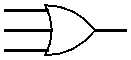
\includegraphics[width=0.2\textwidth]{or-gate-3-inputs}
		\end{figure}
		\item Given inputs A,B,C, and output Y, the equation would be $Y=A\oplus B\oplus C$. The truth table and symbol are below:
		\begin{figure}[h]
			\centering
			\begin{tabular}{|ccc|c|}
				\hline
				A & B & C & Y \\
				\hline
				0 & 0 & 0 & 0 \\
				0 & 0 & 1 & 1 \\
				0 & 1 & 0 & 1 \\
				0 & 1 & 1 & 0 \\
				1 & 0 & 0 & 1 \\
				1 & 0 & 1 & 0 \\
				1 & 1 & 0 & 0 \\
				1 & 1 & 1 & 0 \\
				\hline
			\end{tabular}
			\quad\quad
			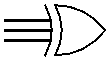
\includegraphics[width=0.2\textwidth]{xor-gate-3-inputs}
		\end{figure}
		\item Given inputs A,B,C, D and output Y, the equation would be $Y=\overline{A\oplus B\oplus C \oplus D}$. The truth table and symbol are below:
		\begin{figure}[h]
			\centering
			\begin{tabular}{|cccc|c|}
				\hline
				A & B & C & D &Y \\
				\hline
				0 & 0 & 0 & 0 & 1 \\
				0 & 0 & 0 & 1 & 0 \\
				0 & 0 & 1 & 0 & 0 \\
				0 & 0 & 1 & 1 & 1 \\
				0 & 1 & 0 & 0 & 0 \\
				0 & 1 & 0 & 1 & 1 \\
				0 & 1 & 1 & 0 & 1 \\
				0 & 1 & 1 & 1 & 1 \\
				1 & 0 & 0 & 0 & 0 \\
				1 & 0 & 0 & 1 & 1 \\
				1 & 0 & 1 & 0 & 1 \\
				1 & 0 & 1 & 1 & 1 \\
				1 & 1 & 0 & 0 & 1 \\
				1 & 1 & 0 & 1 & 1 \\
				1 & 1 & 1 & 0 & 1 \\
				1 & 1 & 1 & 1 & 1 \\
				\hline
			\end{tabular}
			\quad\quad
			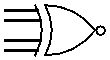
\includegraphics[width=0.2\textwidth]{xnor-gate-4-inputs}
		\end{figure}
	\end{enumerate}
\end{sol}

\begin{ex}{1.77}
	How many different truth tables exist for Boolean functions of $N$ variables.?
\end{ex}

\begin{sol}\
	When $N=2$, the result is $16$. The reason is that an input is a pair $(A, B)$, and there are 4 such pairs, and hence 4 unique outputs. Since each output is 0 or 1, this means there are $2^4$ unique functions. If $N=3$, there are $2^{3}$ possible outputs, and hence $2^{8}$ possible functions. In general, there are $2^{2^N}$ Boolean functions of $N$ variables.
\end{sol}

\begin{ex}{1.78}
	Is it possible to assign logic levels so that a device with the transfer characteristics shown in Figure~\ref{1-78} would serve as an inverter? If so,what are the input and output low and high levels ($V_{IL}, V_{OL}, V_{IH}$, and $V_{OH}$) and noise margins ($NM_{L}$ and $NM_H$)? If not, explain why not.
	\begin{figure}
		\centering
		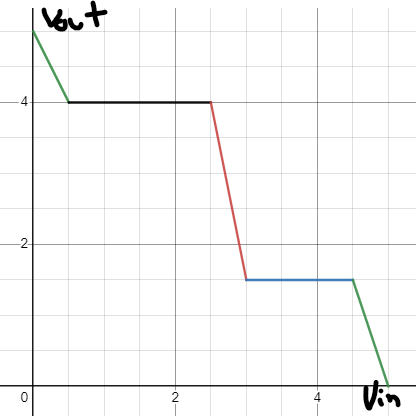
\includegraphics[width=0.3\textwidth]{exercise-78}
		\caption{DC Transfer Characteristics: Exercise 1-78}
		\label{1-78}
	\end{figure}
\end{ex}

\begin{sol}
	Yes. We can choose $V_{OH}=4$, $V_{IH}=3$, $V_{IL}=\frac{5}{2}$, and $V_{OL}=\frac{3}{2}$. Then $NM_{H}=NM_{L}=1$.
\end{sol}

\begin{ex}{1.79}
	Repeat Exercise 1.78 for the transfer characteristics shown in Figure
	\begin{figure}
		\centering
		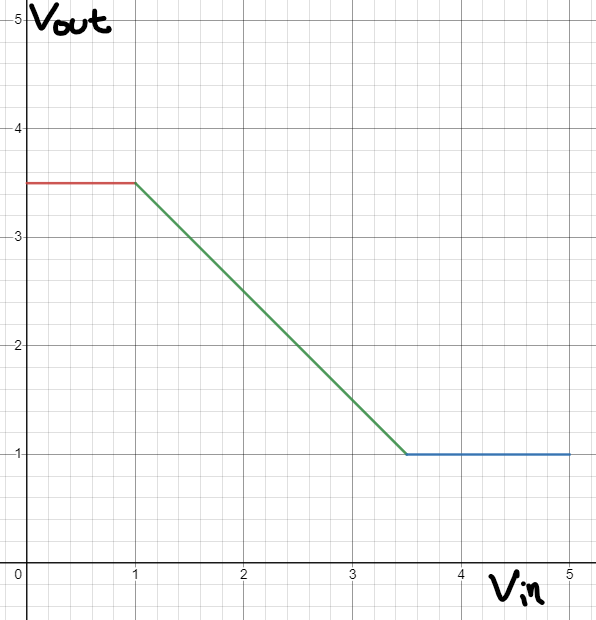
\includegraphics[width=0.3\textwidth]{exercise-1-79-transfer-characteristics}
		\caption{DC Transfer Characteristics: Exercise 1-79}
		\label{1-79}
	\end{figure}
\end{ex}

\begin{sol}
	Because the slope of the transfer characteristics is never better than $-1$, the system does not have gain. Put another way, we require $V_{OL}<V_{IL}$ and $V_{OH}>V_{IH}$, but here they would be equal.
\end{sol}

% --------------------------------------------------------------
%     You don't have to mess with anything below this line.
% --------------------------------------------------------------

\end{document}